% Page 017 — page imprimée 13
% Pierre Bertrand, le galérien de Campis
% Reconstruction éditoriale en LaTeX.

{\fontsize{10.2}{12.1}\selectfont

\begin{center}
{\bfseries\large Pierre Bertrand, le galérien de Campis}
\end{center}

Les prédicants et gens recherchés pour cause de religion étaient assurés de trouver refuge, à Campis dans la maison Bertrand.

\begin{quote}
\itshape
« Après Vivent un des premiers prédicants, ce furent Rey de Massevaques, un voisin, Plan de St Martin de Corconac près de l’Estrechure et sans doute d’autres dont on n’a pas gardé le souvenir ; ils font laver leur linge à Campis et laissent dans une cache armes et sermons. Pierre Bertrand, fils de la famille se fait le guide, en particulier de Roman qui a procédé dans la maison à un baptême ainsi qu’au mariage de son hôte avec Marie Carteirade de Ferrussac.

Le 29 Septembre 1697 ... Roman, accompagné de Rey, tient une assemblée au Crouzet, dans la même région, chez Guillaume Cabanel : deux cents personnes l’écoutent tandis que la maison est gardée par des hommes en armes. Mais on a remarqué, le jour même, à la foire de Meyrueis, l’absence de tous les habitants de Campis qui ont préféré se ménager pour leur course nocturne ; dans ces vallons qui descendent de l’Aigoual à Meyrueis un traître veille à Pourcarès, Poujol : contre argent il trahit Roman et Bertrand. Roman qu’une chance parfois insolente a protégé jusqu’au bout, échappe à ses dénonciations ; Bertrand passe à la clandestinité, mais il est arrêté peu après et condamné aux galères au début de 1698, à l’âge de 22 ans. »
\end{quote}

Voici d’ailleurs l’extrait du registre d’écrou concernant Pierre Bertrand, amené de Montpellier « par un archer et trois fuzilliers » en compagnie de trois autres religionnaires dont David Laget, cardeur de laine, de Massevaques près de Cabrillac... Il était également considéré comme « avertisseur » d’assemblée.

\vspace{0.25em}

N° 21504 -- Pierre Bertrand fils de David et de Marie Lagar, laboureur, natif de Campy en Cévennes, âgé de 22 ans, bonne taille, cheveux châtains, visage rond, de la RPR \textbf{condamné pour assemblées, à vie}. Affecté à la galère \textit{La grande Réale} à Marseille.

Mention marginale : Mort à l’hospitale le 21\textsuperscript{e} août 1705.

\vspace{0.2em}

\begin{flushright}
\textsuperscript{*} Philippe Chambon dans « Itinéraires Protestants en Languedoc » p. 74
\end{flushright}

\vspace{0.15em}

\begin{center}
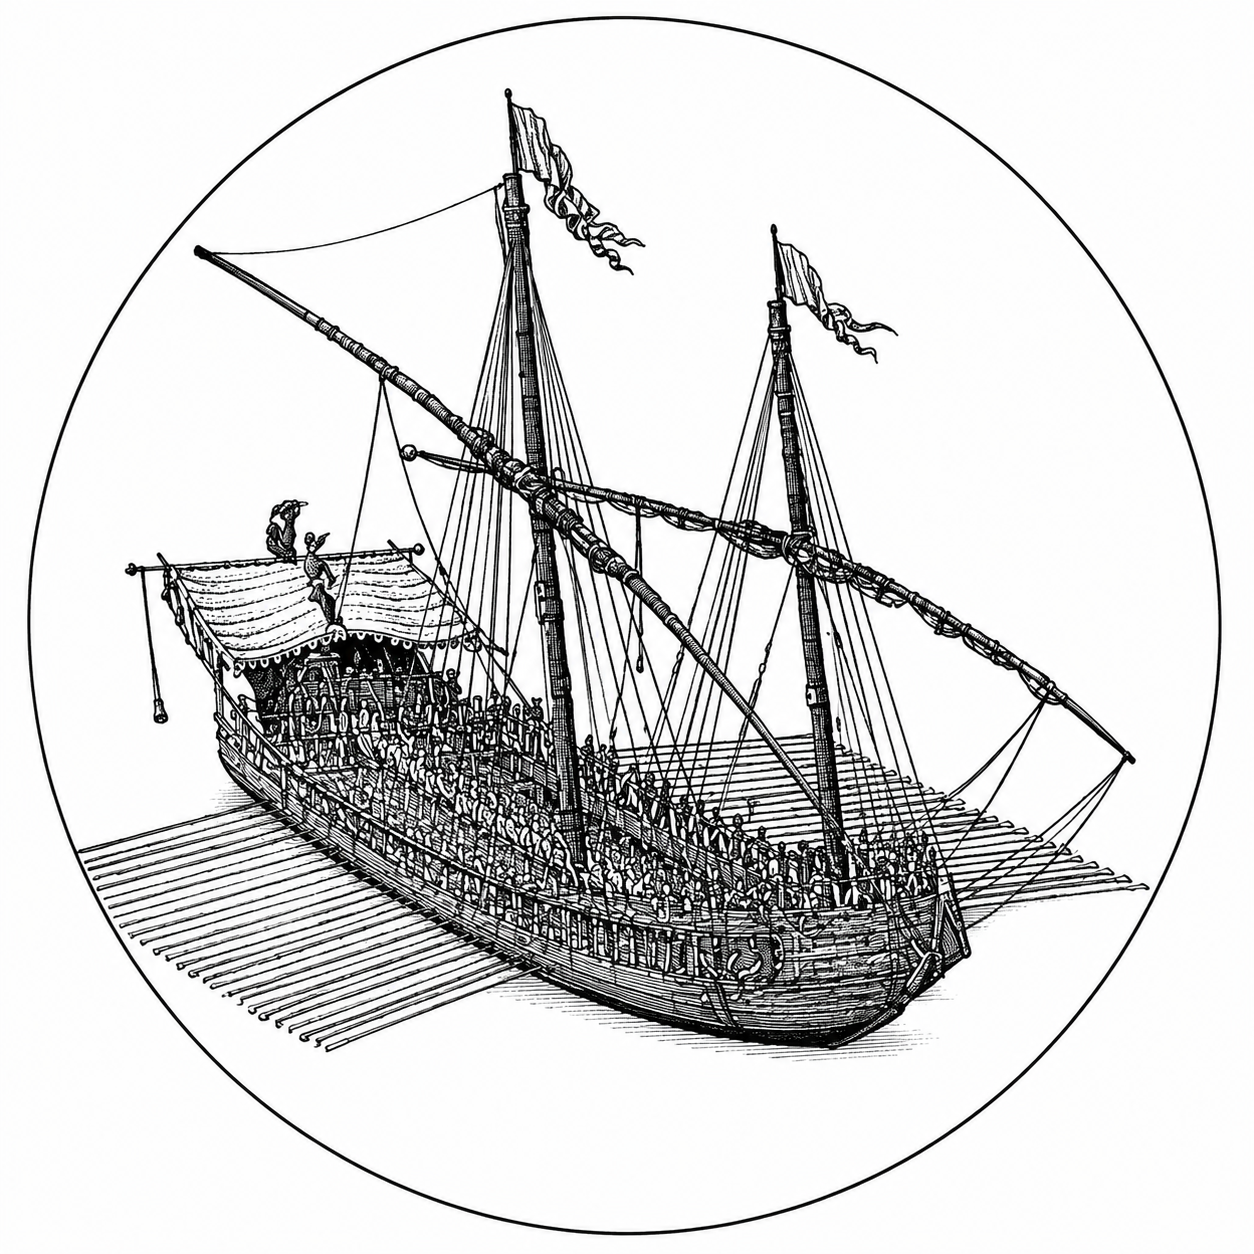
\includegraphics[width=0.72\textwidth]{imgs/017.png}
\end{center}

}

